\documentclass[12pt]{article}
\usepackage{setspace, amsmath, mathdots, amssymb, graphicx, multirow, gensymb, slashbox}
\usepackage[margin=1.5in]{geometry}
\onehalfspacing

\begin{document}
\noindent STA 250 Homework 1 \newline Yichuan Wang \newline \newline
\textbf{Problem 1} \newline
(a) Since the Gibbs sampler generates a Markov chain, as $t \rightarrow \infty$, we have $P(X_1^{(t+1)} = x_1 | X_2^{(t)} = x_2) \rightarrow p(x_1|x_2)$. Also we may assume the Markov chain is ergodic, hence $P(X_1^{(t)} = x_1) \rightarrow \pi(x_1), P(X_2^{(t)} = x_2) \rightarrow \pi(x_2)$.
\newline
\newline
\textbf{Problem 2} \newline
(i)
\begin{center}
	$Y_i|\beta \sim \text{Binomial}(m_i, \text{logit}^{-1}(x_i^T\beta)), \beta \in \mathbb{R}^p$
\end{center}
So we have
\begin{align*}
	p(y_i|\beta) &= {m_i \choose y_i}(\frac{e^{x_i^T\beta}}{1+e^{x_i^T\beta}})^{y_i}(1 - \frac{e^{x_i^T\beta}}{1+e^{x_i^T\beta}})^{m_i - y_i} \\
	&= {m_i \choose y_i}\frac{e^{(x_i^T\beta)y_i}}{(1+e^{x_i^T\beta})^{m_i}}
\end{align*}
Then
\begin{align*}
	p(\mathbf{y}|\beta) \propto \frac{\exp({\sum_{i=1}^n(x_i^T\beta)y_i})}{\prod_{i=1}^n (1+e^{x_i^T\beta})^{m_i}}
\end{align*}
and
\begin{align*}
	p(\beta) \propto \exp[-\frac{1}{2}(\beta - \mu_0)^T \Sigma_0^{-1} (\beta - \mu_0)]
\end{align*}
So the posterior is, up to proportionality
\begin{align*}
	p(\beta|\mathbf{y}) \propto \frac{\exp[\sum_{i=1}^n(x_i^T\beta)y_i - \frac{1}{2}(\beta - \mu_0)^T \Sigma_0^{-1} (\beta - \mu_0)]}{\prod_{i=1}^n (1+e^{x_i^T\beta})^{m_i}}
\end{align*}
We may take logarithm of the proportional posterior for calculation, which is
\begin{align*}
	\sum_{i=1}^n(x_i^T\beta)y_i - \frac{1}{2}(\beta - \mu_0)^T \Sigma_0^{-1} (\beta - \mu_0) - \sum_{i=1}^n m_i \log(1+e^{x_i^T\beta})
\end{align*}
(ii) In this problem, I used the Metropolis-Hastings-within-Gibbs to generate the Markov chain for posterior distribution. The proposal distribution was
\begin{align*}
	\begin{pmatrix} \beta_0^{(t)} \\ \beta_1^{(t)} \end{pmatrix} | \begin{pmatrix} \beta_0^{(t-1)} \\ \beta_1^{(t-1)} \end{pmatrix} \sim 					N(\begin{pmatrix} \beta_0^{(t-1)} \\ \beta_1^{(t-1)} \end{pmatrix}, \begin{pmatrix} v_0 & 0 \\ 0 & v_1 \end{pmatrix}) \\
\end{align*}
The algorithm was performed as the following: \newline
(1) Set initial values $\beta_0^{(0)} = 0, \beta_1^{(0)} = 0, t = 0, v_0 = v_1 = 1$. \newline
(2) Let $\beta_0^{(t+1)} = \beta_0^{(t)}, \beta_1^{(t+1)} = \beta_1^{(t)}$, sample $\beta_0^{(t+1)}$ from $N(\beta_0^{(t)}, v_0)$. \newline
(3) Compute the logarithm posterior of $\begin{pmatrix} \beta_0^{(t+1)} \\ \beta_1^{(t+1)} \end{pmatrix} | \begin{pmatrix} \beta_0^{(t)} \\ \beta_1^{(t)} \end{pmatrix}$, $\log \pi(\beta^{(t+1)}|\beta^{(t)})$, as well as the logarithm posterior of $\begin{pmatrix} \beta_0^{(t)} \\ \beta_1^{(t)} \end{pmatrix} | \begin{pmatrix} \beta_0^{(t+1)} \\ \beta_1^{(t+1)} \end{pmatrix}$, $\log \pi(\beta^{(t)}|\beta^{(t+1)})$. \newline
(4) Since we are using a symmetric proposal distribution, we have $\log\alpha = \log \pi(\beta^{(t)}|\beta^{(t-1)}) - \log \pi(\beta^{(t-1)}|\beta^{(t)})$.
(5) According to MH algorithm, when $\alpha > 1$, we always accept sample; when $\alpha < 1$, we accept with probability $\alpha$. \newline
(6) After updating (accepting or rejecting sample) $\beta_0^{(t+1)}$, we sample $\beta_1^{(t+1)}$ from $N(\beta_1^{(t)}, v_1)$ and repeat steps (3) to (5) to update it. \newline
(7) Set $t = t+1$, repeat steps (2) through (6) until desired iterations or convergence. \newline
For each dataset, 10000 iterations were executed and the first 1000 were considered as "burnin" period, during which retuning was performed at every $100^{th}$ iteration: if the acceptance rate for either parameter is too low (less than 20\%), the variance $v_j$ would be divided by 1.1; if the rate is too high (greater than 60\%), the variance would be multiplied by 1.1. \newline
(iii) The following table and graph display the coverage property based on results from Gauss:
\begin{table}[ht]
\centering
\begin{tabular}{rrr}
  \hline
 & beta\_0 & beta\_1 \\ 
  \hline
p\_01 & 0.01 & 0.01 \\ 
  p\_05 & 0.07 & 0.03 \\ 
  p\_10 & 0.10 & 0.06 \\ 
  p\_25 & 0.27 & 0.20 \\ 
  p\_50 & 0.52 & 0.48 \\ 
  p\_75 & 0.76 & 0.77 \\ 
  p\_90 & 0.92 & 0.88 \\ 
  p\_95 & 0.94 & 0.95 \\ 
  p\_99 & 0.99 & 0.99 \\ 
   \hline
\end{tabular}
\end{table}
\newline
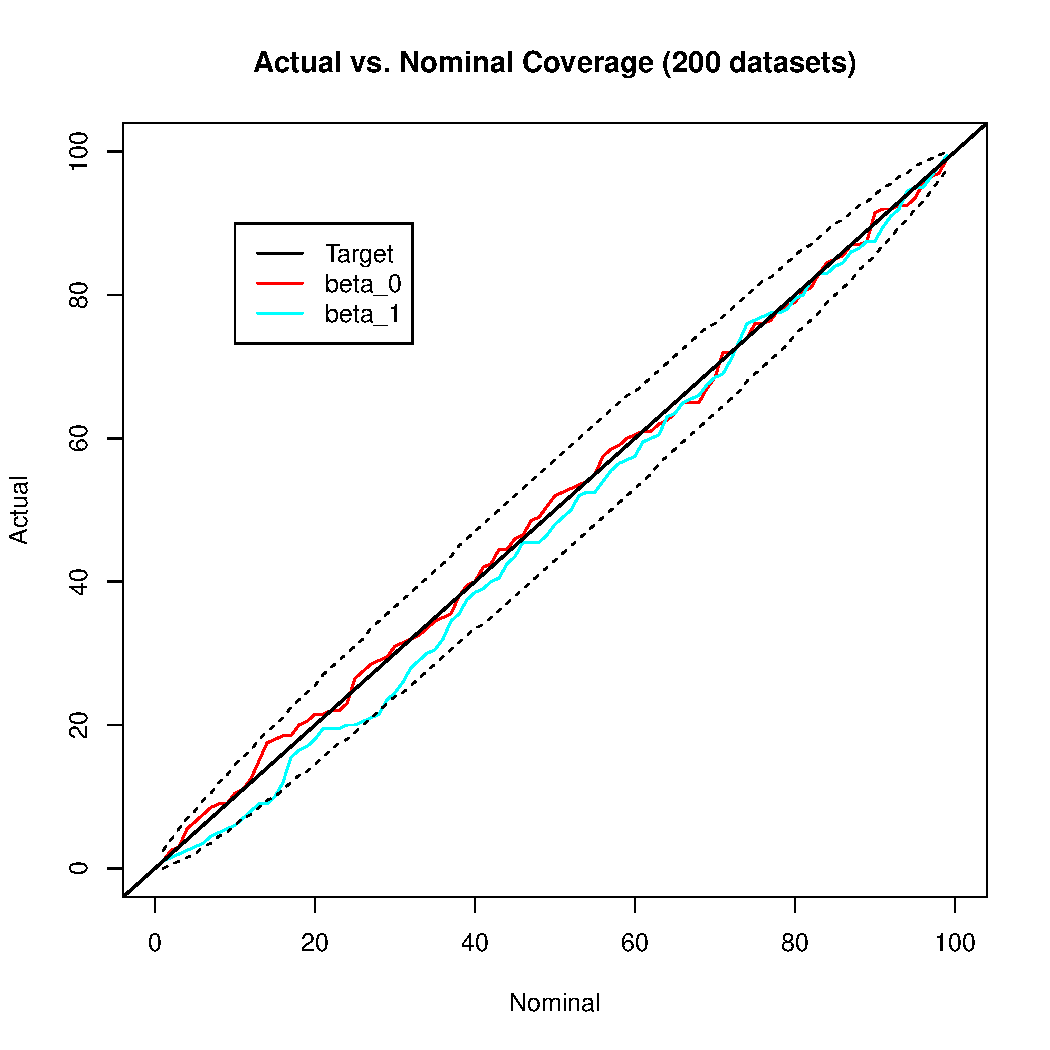
\includegraphics[width=\textwidth]{coverage_line_plot.pdf}








\end{document}